% This is text associated with the open textbook "Open Electromagnetics"
% See immediately below for author, date
% This work is licensed under the Creative Commons Attribution-ShareAlike 4.0 International License. (CC BY-SA 4.0) 
% To view a copy of the license, visit http://creativecommons.org/licenses/by-sa/4.0/

%ORB TITLE Magnetic Field of a Toroidal Coil
%ORB AUTHOR 0        # S.W. Ellingson, Virginia Tech (ellingson@vt.edu)
%ORB DATE 20180806   # yyyymmdd
%ORB ABSTRACT Magnetic Field of a toroidal coil

\label{m0049_Magnetic_Field_of_a_Toroidal_Coil} % <-- Must match name of this file and module directory name.  Don't mess with this!
\index{toroidal coil|(}

A toroid 
\index{toroid}
is a cylinder in which the ends are joined to form a closed loop.
An example of a toroidal coil 
\index{coil!toroidal|see{toroidal coil}}
is shown in Figure~\ref{m0049_fToroidalCoilExample}.
Toroidal coils are commonly used to form inductors and transformers.
The principal advantage of toroidal coils over straight coils in these applications is \emph{magnetic field containment} -- as we shall see in this section, the magnetic field outside of a toroidal coil can be made negligibly small.
This reduces concern about interactions between this field and other fields and structures in the vicinity.
%
\begin{figure}[b!]
\begin{center}
\pdftooltip{{  % note double braces
\includegraphics[width=2in]{modules/m0049_fToroidalCoilExample.eps}
% https://en.wikipedia.org/wiki/File:3Com_OfficeConnect_ADSL_Wireless_11g_Firewall_Router_2012-10-28-0869.jpg
}}{A photo of a toroidal coil on a circuit board. Wire is wound on a yellow plastic toroid. Beside the coil are two cylindrical capacitors.}
\end{center} 
\centerline{\scriptsize 
\copyright~\hyperref[m0049_fToroidalCoilExample_Credit]{Slick} 
\href{https://creativecommons.org/publicdomain/zero/1.0/deed.en}{CC0 1.0} 
} 
\caption{
\label{m0049_fToroidalCoilExample}
A toroidal coil used as a large-value inductor in the power supply of a wireless router.
}
\end{figure} 

In this section, we use the magnetostatic form of Ampere's Circuital Law (ACL) 
\index{Ampere's law!magnetostatics}
(Section~\ref{m0019_Amperes_Law_Magnetostatics}) to determine the magnetic field due to a steady (DC) current flowing through a toroidal coil.
The problem is illustrated in Figure~\ref{m0049_fToroidalCoil}.
The toroid is circular with inner and outer radii $a$ and $b$, respectively. %; and with circular cross-section having radius $c=(b-a)/2$.
The coil consists of $N$ windings (turns) of wire wound with uniform winding density.
This problem is easiest to work in cylindrical coordinates with the toroid centered on the origin in $z=0$ plane.
%
\begin{figure}
\begin{center}
\pdftooltip{{  % note double braces
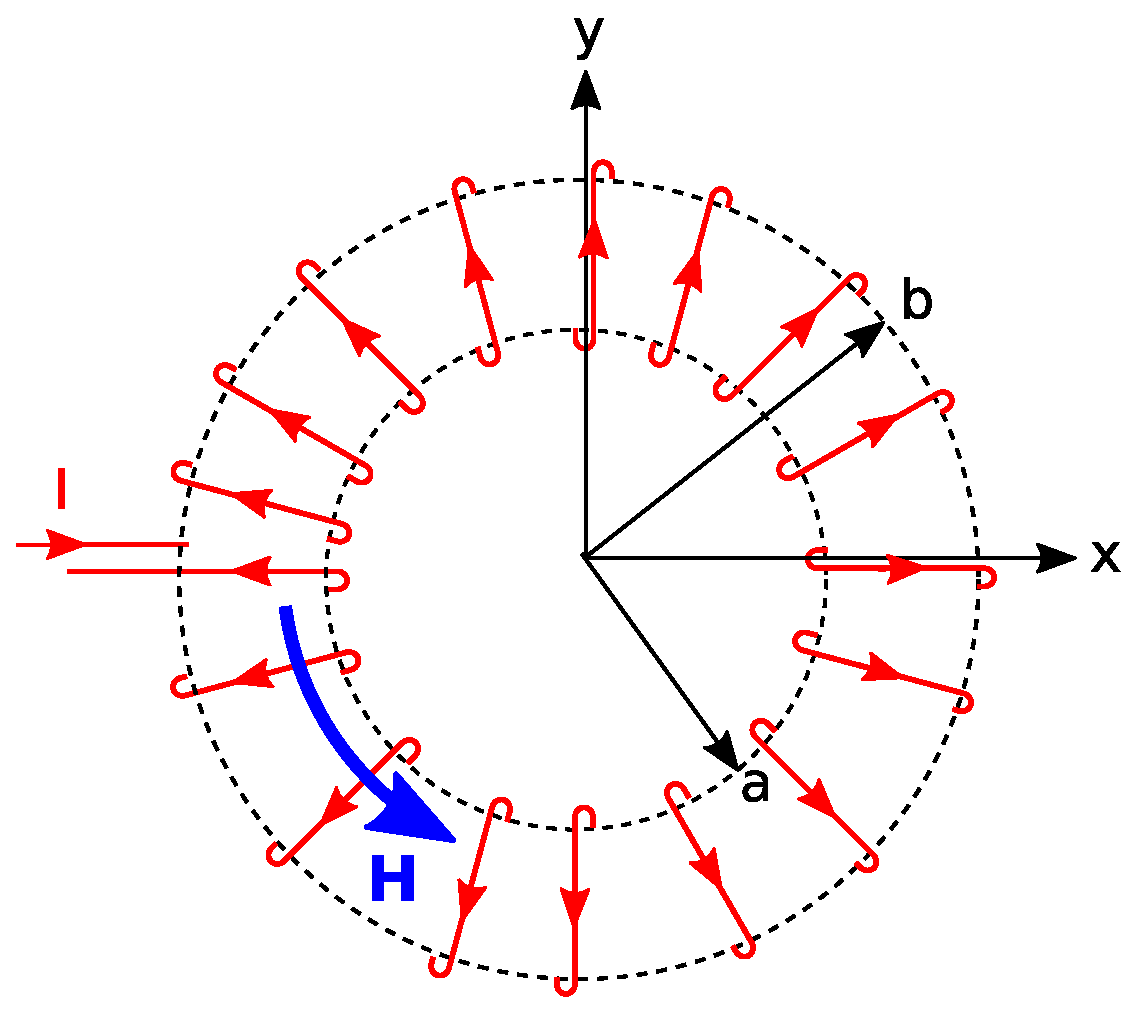
\includegraphics[width=\columnwidth]{modules/m0049_fCoil.eps}
}}{A circular toroidal coil, with the open center at the origin of a xy-axis, with inner radius a and outer radius b. Around the loop the coil is shown as looped arrows, each of which are pointing out away from the center of the coil. From the left, a vector labeled I is pointing toward the coil. H is shown counterclockwise around the loop.}
\end{center} 
% ***WikipediaCommonsURL
%\centerline{\scriptsize 
%\copyright~\hyperref[m0049_fCoil_Credit]{author} 
%\href{https://creativecommons.org/licenses/by-sa/4.0/}{CC BY-SA 4.0} 
%} 
\caption{
\label{m0049_fToroidalCoil}
Geometry of a toroidal coil.
}
\end{figure}  

To begin, let's take stock of what we already know about the answer, which is actually quite a bit.
First, a review of 
Section~\ref{m0120_Magnetic_Field_of_a_Coil} (``Magnetic Field Inside a Straight Coil'') is recommended.
There it is shown that the magnetic field deep inside a straight coil is aligned with axis of the coil.
This can be explained using the result for the magnetic field due to a straight line current (Section~\ref{m0119_Magnetic_Field_of_a_Long_Wire}), in which we found that the magnetic field follows a ``right-hand rule'' -- 
\index{right-hand rule!magnetic field of a wire}
The magnetic field points in the direction of the curled fingers of the right hand when the thumb of the right hand is aligned in the direction of current flow. 
The wire comprising the coil is obviously \emph{not} straight, but we can consider just one short segment of one turn and then sum the results for all such segments.
When we do this, we see that the direction of the magnetic field inside the coil must be in the $+\hat{\bf \phi}$ direction when the current $I$ is applied as shown in Figure~\ref{m0049_fToroidalCoil}.
Also, because the problem is identical after any amount of rotation around the $z$ axis, the magnitude of the magnetic field cannot depend on $\phi$.
Putting these findings together, we find that the most general form for the magnetic field intensity inside or outside the coil is ${\bf H}=\hat{\bf \phi}H(\rho,z)$.  

Here's the relevant form of ACL:
%
\begin{equation}   
\oint_{\mathcal C}{ {\bf H} \cdot d{\bf l} } = I_{encl}  
\label{m0049_eACL}
\end{equation}
%
where $I_{encl}$ is the current enclosed by the closed path ${\mathcal C}$.
ACL works for {\it any} closed path, but we need one that encloses some current so as to obtain a relationship between $I$ and ${\bf H}$.
Also, for simplicity, we prefer a path that lies on a constant-coordinate surface.
The selected path is a circle of radius $\rho$ centered on the origin in the $z=z_0$ plane, as shown in Figure~\ref{m0049_fPath}.
We further require ${\mathcal C}$ to lie entirely inside the coil, which ensures that the enclosed current includes the current of all the windings as they pass through the hole at the center of the toroid.
We choose the direction of integration to be in the $+\phi$ direction, which is consistent with the indicated direction of positive $I$.
That is, when $I$ is positive, the current in the windings of the coil pass through the surface bounded by ${\mathcal C}$ in the same direction as the curled fingers of the right hand when the thumb is aligned in the indicated direction of ${\mathcal C}$. 
%
\begin{figure}
\begin{center}
\pdftooltip{{  % note double braces
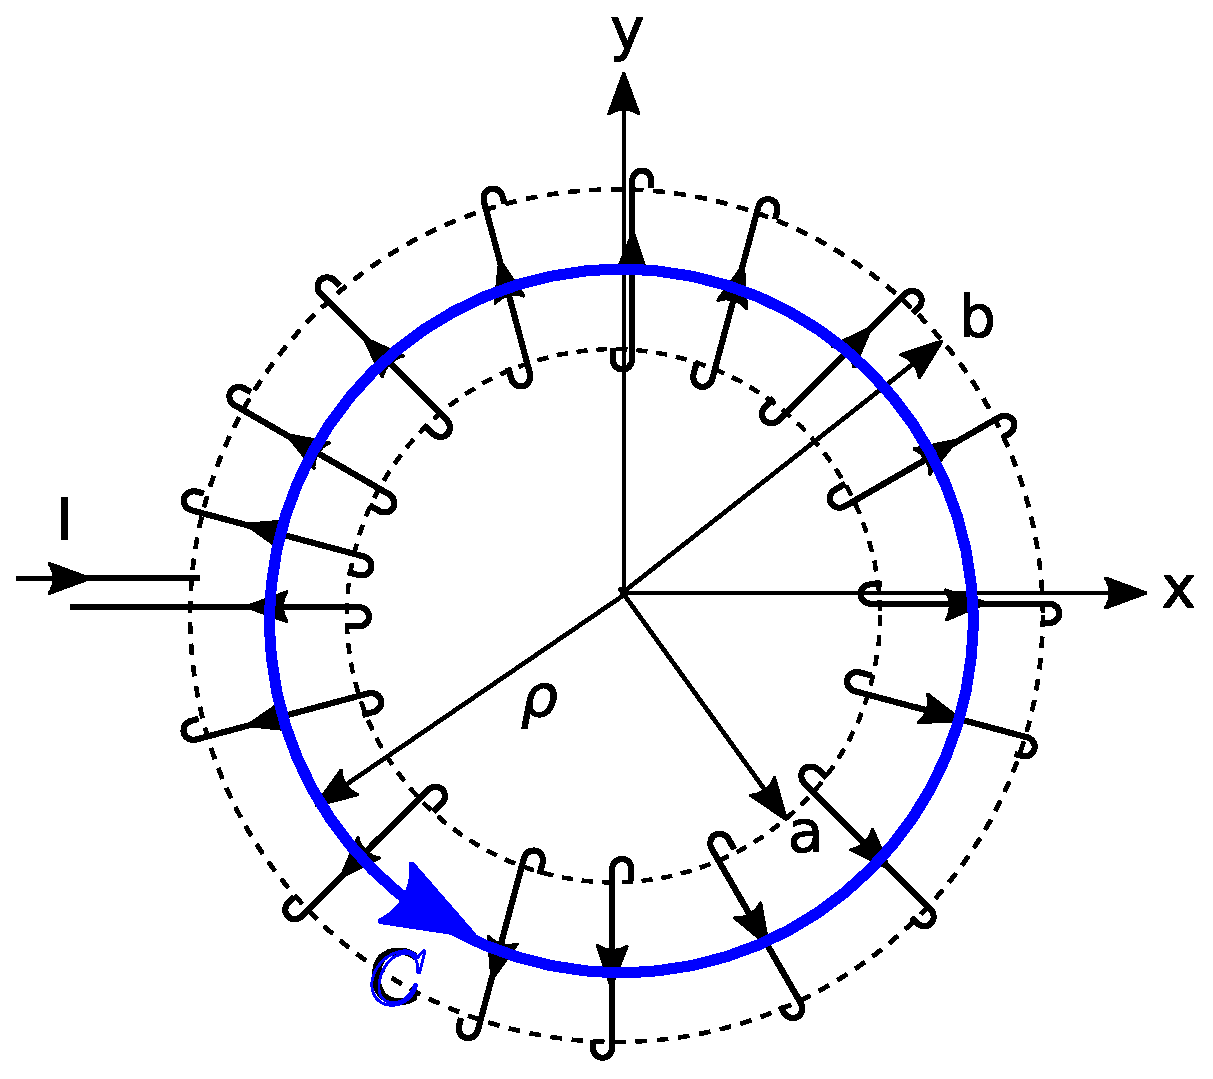
\includegraphics[width=\columnwidth]{modules/m0049_fPath.eps}
}}{A circular toroidal coil, the same as in a previous figure. From the origin pointing toward the bottom left, is a vector labeled rho. A blue circle sits in the middle of the coil, with an arrow pointed in a counterclockwise direction, labeled C.}
\end{center} 
% ***WikipediaCommonsURL
%\centerline{\scriptsize 
%\copyright~\hyperref[m0049_fPath_Credit]{author} 
%\href{https://creativecommons.org/licenses/by-sa/4.0/}{CC BY-SA 4.0} 
%} 
\caption{
\label{m0049_fPath}
Selected path of integration.
}
\end{figure}  

In terms of the variables we have defined, the enclosed current is simply
%
\begin{equation}
I_{encl}=NI
\end{equation}
% 
Equation~\ref{m0049_eACL} becomes
%
\begin{equation}   
\oint_{\mathcal C}{ \left[\hat{\bf \phi}H(\rho,z_0)\right] \cdot d{\bf l} } = NI 
\label{m0049_eACL1}
\end{equation}
%
Now evaluating the integral:
%
\begin{flalign}   
NI &= \int_{0}^{2\pi}{ \left[\hat{\bf \phi}H(\rho,z_0)\right] \cdot \left(\hat{\bf \phi}~\rho~d\phi\right) } \nonumber \\
   &= \rho H(\rho,z_0) \int_{0}^{2\pi}{ d\phi }                                                       \nonumber \\
   &= 2\pi\rho H(\rho,z_0)                                                                   
\label{m0049_eACL2}
\end{flalign}
%
It is now clear that the result is independent of $z_0$. 
Summarizing:
%
\begin{equation}
\boxed{
{\bf H} = \hat{\bf \phi}\frac{NI}{2\pi\rho} ~~ \mbox{inside coil}
}
\label{m0049_eResult}
\end{equation}

Let's take a moment to consider the implications of this result.
%
\begin{itemize}
\item Note that it is dimensionally correct; that is, current divided by the circumference of ${\mathcal C}$ ($2\pi\rho$) gives units of A/m, which are the units of ${\bf H}$. 
\item We have found that the magnetic field is proportional to winding density (i.e., number of windings divided by circumference) times current. To increase the magnetic field you can either use more windings or increase the current.
\item Remarkably, we have found that the magnitude of the magnetic field inside the coil depends only on $\rho$; i.e., the distance from the central (here, $z$) axis.  It is independent of $z$.
\end{itemize}
%
Summarizing:
%
%ORB HIGHLIGHT
\begin{mdframed}[backgroundcolor=yellow!20,nobreak=true] 
The magnetic field inside a toroidal coil (Equation~\ref{m0049_eResult}) depends only on distance from the central axis and is proportional to winding density and current.
\end{mdframed}

Now let us consider what happens outside the coil.  For this, we consider any path of integration (${\mathcal C}$) that lies completely outside the coil.  
Note that any such path encloses no current and therefore $I_{encl}=0$ for any such path.
In this case we have:
%
\begin{equation}   
\oint_{\mathcal C}{ {\bf H} \cdot d{\bf l} } = 0 
\end{equation}
%
There are two ways this could be true.  Either ${\bf H}$ could be zero everywhere along the path, or ${\bf H}$ could be non-zero along the path in such a way that the integral windings out to be zero.  The radial symmetry of the problem rules out the second possibility -- if ${\bf H}$ is radially symmetric and ${\mathcal C}$ is radially symmetric, then the sign of ${\bf H} \cdot d{\bf l}$ should not change over ${\mathcal C}$.  Therefore:
%
%ORB HIGHLIGHT
\begin{mdframed}[backgroundcolor=yellow!20,nobreak=true,nobreak=true] 
The magnetic field everywhere outside an ideal toroidal coil is zero. 
\end{mdframed}
%
Note the caveat signaled by the use of the adjective ``ideal.'' In a practical toroidal coil, we expect there will be some leakage of magnetic flux between the windings.  In practice, this leakage can be made negligibly small by using a sufficiently high winding density and winding the wire on material on a toroidal form (a ``core'') having sufficiently large permeability.  
The use of a high-permeability core, as shown in Figure~\ref{m0049_fToroidalCoilExample}, will dramatically improve the already pretty-good containment.  In fact, the use of such a core allows the spacing between windings to become quite large before leakage becomes significant.

One final observation about toroidal coils is that at no point in the derivation of the magnetic field did we need to consider the cross-sectional shape of the coil; we merely needed to know whether ${\mathcal C}$ was inside or outside the coil.  Therefore:
%
%ORB HIGHLIGHT
\begin{mdframed}[backgroundcolor=yellow!20,nobreak=true] 
The magnetic field inside an ideal toroidal coil does not depend on the cross-sectional shape of the coil. 
\end{mdframed}

%------------------------------

{\bf Additional Reading:}
\begin{itemize}
\item ``\href{https://en.wikipedia.org/wiki/Toroidal_inductors_and_transformers}{Toroidal Inductors and Transformers}'' on Wikipedia.
\end{itemize}

\index{toroidal coil|)}

